
%======================问题介绍====================================
\section{Introduction}
\subsection{Background}
 As of 1 February 2015, more than 22,000 suspected cases have been 
 reported by the World Health Organization (WHO) and the
numbers continue to rise\cite{who15}.
The exponential increase of Ebola virus disease (EVD) cases in
Sierra Leone, Liberia, and Guinea since the months of
August and September, 2014, defines an unprecedented
health threat to west Africa. 
A massive international
response necessitating the large-scale deployment of
medical resources and non-pharmacological interventions is needed 
to stop the epidemic. 
At current stage, quantitative predictions about the growth 
of the EVD epidemic, the effectiveness of feasible delivery 
systems and the evaluation of quantity of possible vaccine/drag
needed are critical to the eradication. In the mean time, the ongoing 
epidemic, as unfortunate as it is, also offers
to further our insights in the transmission characteristics of EVD, 
as well as effectiveness of non-pharmacological interventions.  
We, therefore, cannot overemphasize the importance of collecting data and 
reproducing mathematical models
 relating to population behaviors and control interventions influencing disease
spread  and how these have changed over
time. In this report, we exploit the data available for the 
current Ebola epidemic, perform detailed analysis, 
model-fitting and forecasting of epidemic 
spread discretely at the district level as well as at a inter-district
 scale utilizing socio-network and geographical data, and 
 determine optimized delivery system and means to strain of EVD.

\subsection{Related work}
\begin{figure}[ht]
\centering
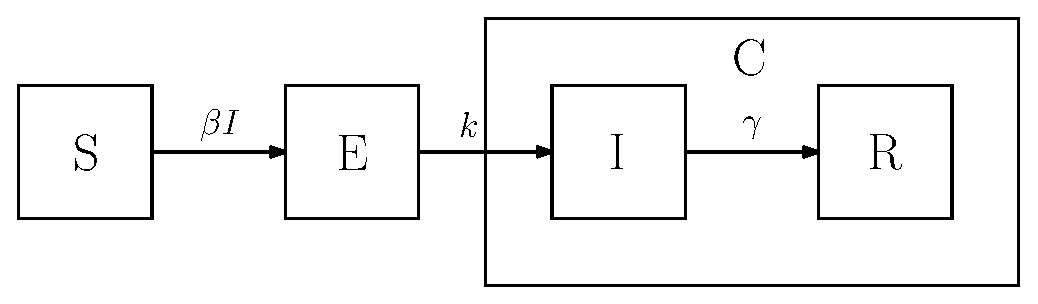
\includegraphics[width=12cm]{nseir}
\caption{A schematic representation of the flow of individuals in naive SEIR epidemic model.} 
\medskip
\small
The way \cite{chow04} formulated their dynamics, where $\beta$ is the transmission 
rate per person per week. $k,\,\gamma$ are effective transformation 
rates for $E$ and $I$ respectively. $C$ is the cumulative number of the infected.
\label{fig:naiveseir}
\end{figure}

In recent years, mathematical modelling on epidemic evolutions, 
 taking on various approaches at very detailed conditions, has been 
tailored to make projections from different perspectives.\par
 Traditional epidemiological analysis is typically based on 
 a prior assumption that all individuals in the considered region
are homogenously mixed and then subdividing into different
 compartments based on the stage of the disease. 
 The classic Susceptible-Infectious-Recovered (SIR) model 
 was firstly conceived and widely used, then variations was developed
 \cite{kerm27}\cite{legr07}. Notably, in the EVD case, 
 Susceptible-Exposed-Infectious-Removed (SEIR) model 
 (\autoref{fig:naiveseir}) is used extensively.
 \cite{chow04} utilized collective data of EVD 
 outbreak in 1995 in Congo and in 2000 in Uganda to model the 
 reproduction number $R_0$ and characterize the transmissive pattern 
 under the influences of Ebola Treatment Centers (ETCs), 
 with a touch of stochastics. Later \cite{leko06}, 
 again based on Congo data, focus on the nature of transitions between 
 related compartments in concert with Markov chain Monte Carlo 
 (MCMC) methods, which revealed unobserved features but suffered 
 considerable deviation problem.\par
 
 The SIR model has become detailed enough if not suffers a prior 
 homogenous mixing assumption, and insights on that social-network
 and disease propagation are closely correlated was exploited\cite{newm99}.
 Early work utilized bond and site percolation theory with 
 realizations of ``clustering'' and ``small-world'' effect reflected by 
 real populations\cite{moor00}. Howerver, most results were only 
 presented at the threshold point rather than a realistic model 
 due to the complexity of data collection and computation. Later 
 \cite{meye05} came up with a less theoretical model, capturing an 
 outbreak dynamically in 2002 in Hong Kong and Canada and 
 assessing public health strategies. 
 The network model offers more than unique quantitative insights if
not with a caveat of static nature, that is, it presumes a static
contact pattern throughout the disease propagation. \par
 
\subsection{Restatement of the problem}


%==================================模型建立==============================================
\section{Methods}
\cite{kerm27}
\cite{who152}
\subsection{Construction of SEIR-based model}
Our model of the spread of the EVD is mainly based on the SEIR epidemic model, which will be applied to every single administrative district respectively, with considerations of vaccination, usage of drugs, ETCs, interactions between districts and etc. In order to figure out infections in a certain district caused by its adjacent districts, theories of networks in the graph theory are introduced in our SEIR-based model.

\subsubsection{Assumptions}
\begin{enumerate}
\item Despite the fact that there are several kinds of EVD, we treat all of them as a single kind.
\item One cannot skip the stage of being "Exposed"(E) to become "Infectious"(I).
\item Vaccination is effective for both "Susceptible"(S) and "Exposed"(E), letting them become "Removed"(R).
\item Drugs are only distributed to the "Infectious"(I).
\item Only the people in group "Infectious"(I) will die of EVD.
\item ETCs take in and cure the "Infectious"(I), thus having a positive effect on the transition from (I) to (R), along with a negative effect on the transition from (S) to (E). These effects vary with time due to newly established ETCs and improvement in treatments.
%\item EVD's incubation period and the rate of EVD-caused death are identical in all districts.
\item Natural death and birth are not taken into account.
\item Migration between districts is not taken into consideration, either.
\item The total population ($S+E+I+R$) remains constant.
\end{enumerate}

\subsubsection{Notations}

\begin{table}[h!]
\caption{Notations used}
\label{t:notass}
\medskip
\centering
\begin{tabular}{c c}
\hline
Definition & Symbol \\ [0.5ex]
\hline
the number of Susceptible people & $S(t)$ \\
the number of Exposed people & $E(t)$ \\
the number of Infectious people & $I(t)$ \\
the number of Removed people & $R(t)$ \\
total population & $N_{0}$ \\
\\
rate of infection within the district & $\lambda$ \\
rate of infection between districts & $\mu$ \\
rate of EVD-caused death & $\beta$ \\
rate of transiting from E to I & $\epsilon $ \\
\\
rate of recovery due to ETC & $\gamma_{E}(t) $ \\
isolation factor due to ETC & $k_{E}(t) $ \\
\\
immunity factor due to vaccination & $V(t)$ \\
recovery factor due to drugs & $D(t)$ \\
\\
adjacency matrix & $\bm{A}$ \\
\hline
\end{tabular}
\end{table}

Elements of adjacent matrix $\bm{A} = (a_{ij})_{n\times n}$ are given by:
\begin{equation}
\label{adjac}
a_{ij}=\begin{cases} 1,&\text{if $i,j$ is adjacent}\\
0,&\text{else}
\end{cases},
\end{equation}

where $i$ or $j$ is the index of a district, n is the total number of all districts.

\subsubsection{The improved SEIR model}
...\par
\begin{figure}[ht]
\small
\centering
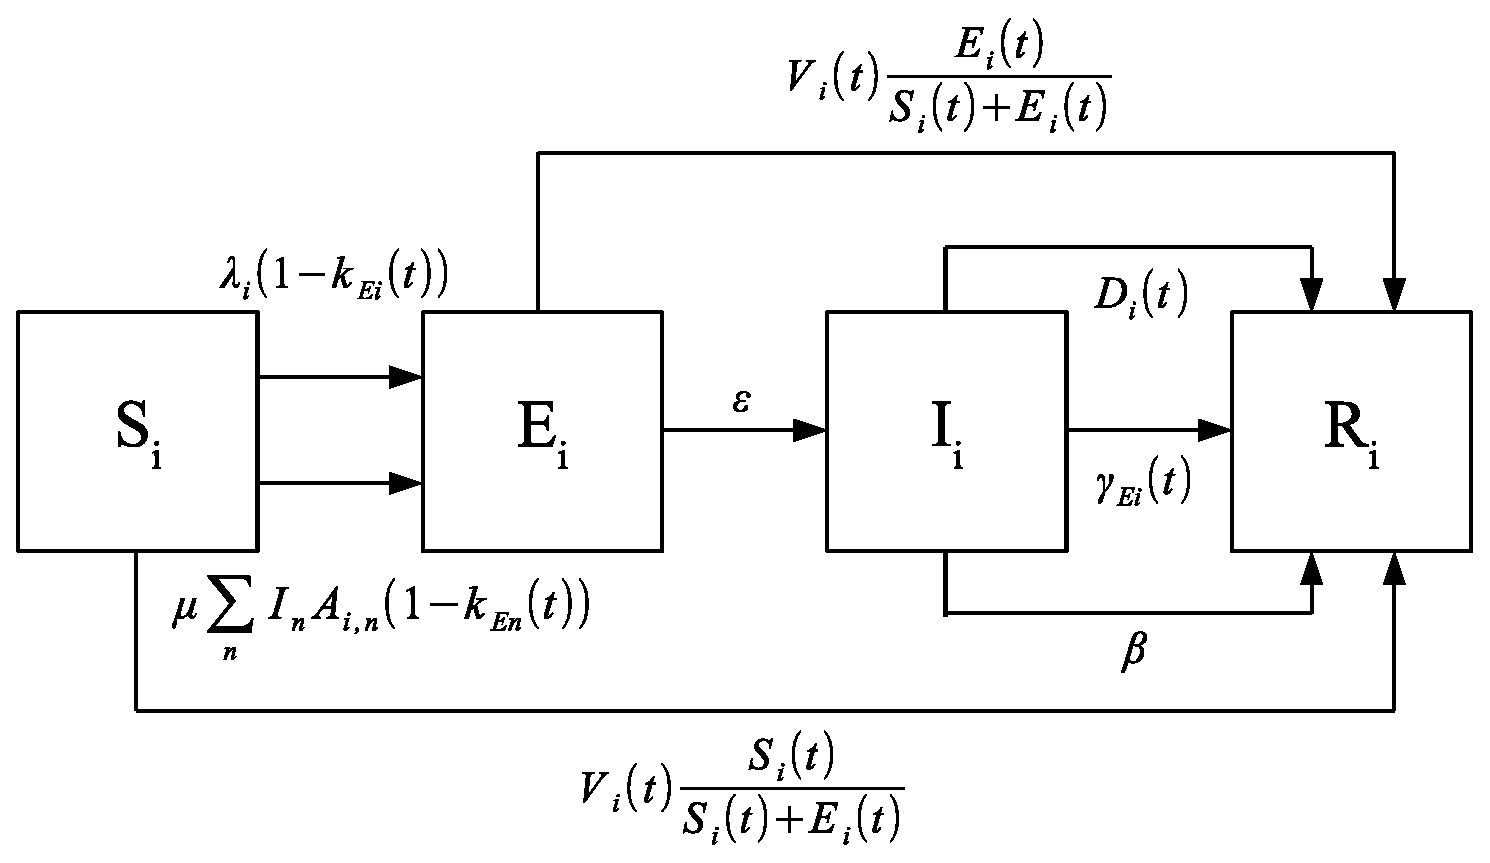
\includegraphics[width=12cm]{aseir}
\caption{A schematic diagram of the flow of individuals in our improved SEIR model.}
\label{fig:Advanced SEIR}
\end{figure}
As showed in \autoref{fig:Advanced SEIR}, the ordinary differential equations for S, E, I and R of a certain district $i$ can be given as followed:



\begin{align}
\dot{S_{i}}(t) &= S_{i}(t)(-\lambda_{i} (1-k_{E,i}(t))  I_{i}(t)  \nonumber\\
\label{eq:seirs}
&\qquad - \mu  \sum_{n} (1-k_{E,n}(t)) A_{i,n} I_{n}(t) - V_{i}(t)  \frac{S_{i}(t)}{S_{i}(t) + E_{i}(t)}) \\
\dot{E}_{i}(t) &= S_{i}(t)(\lambda_{i} (1-k_{E,i}(t))  I_{i}(t)  \nonumber\\
\label{eq:seire}
&\qquad + \mu  \sum_{n} (1-k_{E,n}(t)) A_{i,n} I_{n}(t)) - V_{i}(t)  \frac{E_{i}(t)^2}{S_{i}(t) + E_{i}(t)} - \epsilon E_{i}(t)\\
\label{eq:seiri}
\dot{I}_{i}(t) &= \epsilon E_{i}(t) - {I}_i(t)(D_{i}(t) + \gamma_{E,i}(t) + \beta) \\
\dot{R}_{i}(t) &= V_{i}(t)  \frac{S_{i}(t)^2+E_{i}(t)^2}{S_{i}(t) + E_{i}(t)
}+ {I}_i(t)(D_{i}(t) + \gamma_{E,i}(t) + \beta)
\label{eq:seirr}
\end{align}


%================================PageRank==============================
\subsection{PageRank}
Invented by Larry Page, The algorithm PageRank is originally used by Google Search to rank websites according to their importance. We apply this method to determined the distribution of drugs and vaccines in a country. The introduction of the basic idea will be presented, followed by the justification of the adaption in this problem.

\subsubsection{Simplified algorithm}
The original purpose of PageRank algorithm is to sort the web sites according to the hyperlink between each other. We will begin with a simplified situation with only 4 sites and 8 hyperlinks demonstrated as nodes and arrows as shown in \autoref{fig:a simplified network}.\cite{kard12}
    
\begin{figure}[ht]
\small
\centering
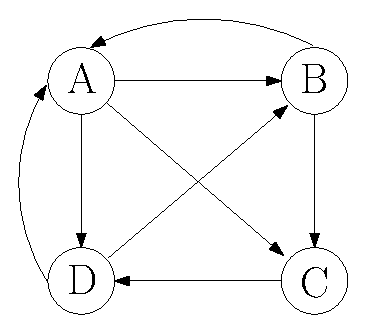
\includegraphics[width=6cm]{pagerankfigure1}
\caption{A simplified network diagram. }
\label{fig:a simplified network}
\end{figure}
    

In order to evaluate the sites, we first have to come up with a data structure to store the relation of between each nodes. PageRank demonstrate the topology of the diagram with the Transition Matrix. For example, the transition matrix of the diagram above is  

\begin{equation}
M = 
\left( \begin{array}{cccc}
0 & 1/2 & 0 & 1/2 \\
1/3 & 0 & 0 & 1/2 \\
1/3 & 1/2 & 0 & 0 \\
1/3 & 0 & 1 & 0 
\end{array} \right)
\end{equation}
           
           
The first row of the matrix $M$ indicate the probability of the transition from A,B,C and D to A, the first column of $v$ indicate the present rank of A,B,C and D. Multiplied by the matrix $M$, $v$ will become a new column vector of a new ranks $M_v$.


\begin{equation}
v = \left( \begin{array}{c}
 1/4 \\
1/4 \\
1/4 \\
1/4 
\end{array} \right),\ \ \ \ 
M_v = 
\left( \begin{array}{c}
 1/4 \\
5/24 \\
5/24 \\
1/3 
\end{array} \right)
\end{equation}
           
           
After iteration, this vector will finally converge at (1/4, 1/4, 1/5, 1/4), which is the ranks of the A,B,C and D. Notice that in the present problem every nodes are interconnected by each other, so that we don't have to deal with the Dead Ends (nodes with no outward links ).

 
\subsubsection{Spider Trap and Smoothing Process}
The Spider Trap represent the node with link to itself as shown in \autoref{fig:Spider Trap}. In actual application the transition matrix would be a highly sparse one which will make it extremely unsmooth. During the iteration the apearance of Spider Trap will even worsen the situation.

\begin{figure}[ht]
\small
\centering
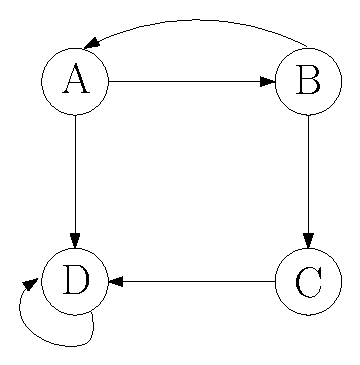
\includegraphics[width=6cm]{spidertrap}
\caption{Spider Trap}
\label{fig:Spider Trap}
\end{figure}

To overcome this problem the PageRank algorithm apply a method called teleporting which allow us teleporting to a random site with a comparatively small probability which is  
The iterative formula with the teleporting is 

\begin{equation}
v\prime=(1-\beta)M_v+e\frac{\beta}{N}
\end{equation}


Normally the $\beta$ will be set as a comparatively small parameter (default is 0.15 in our codes).$e$ is a N-dimensional unit vector to ensure the validity of the formula.In conclution, the effect of the Spider Trap will be significantly eliminated after the iteration following this formula.And therefore, we could finally obtain the reasonable value of pagerank of each nodes.

\subsubsection{Justification for the adaption}

In the present problem, we consider that each districts is connected to each other and we assume that the value of hyperlink between two neighboring districts is proportional to the product of the amount infected people from them. For instance, we apply this method on the determination of the distribution of drugs in Seirra Leone.The final ranks of every districts of today is

\begin{figure}[ht]
\small
\centering
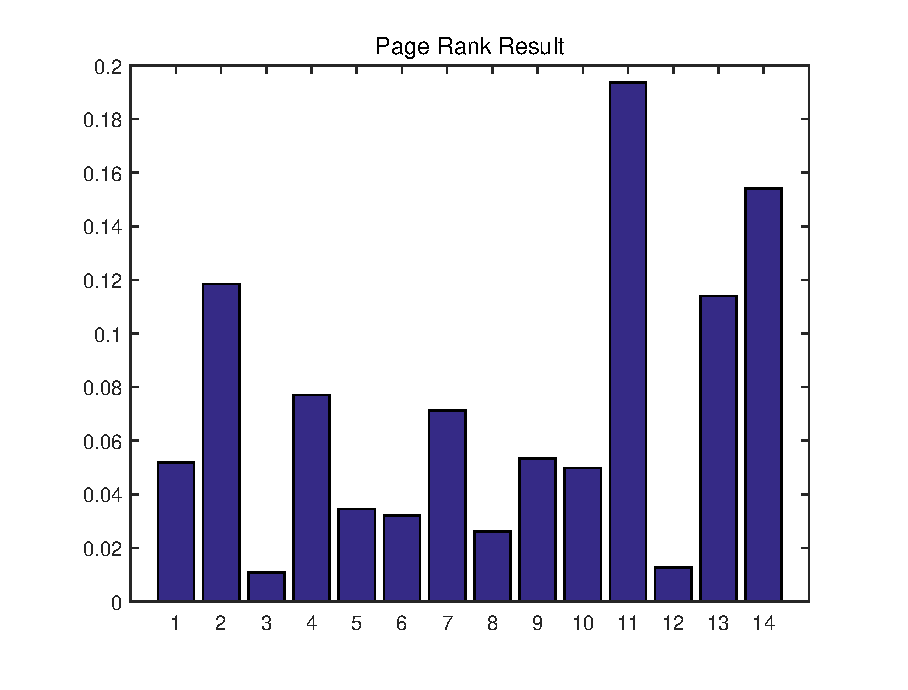
\includegraphics[width=11cm]{demo-pagerankresult}
\caption{PageRank Result}
\label{fig:PageRank Result}
\end{figure}

In \autoref{fig:PageRank Result}, the normalized ranks will determine the proportion of the drugs in each district. In conclution, we calculated the distribution of drugs and vaccines with the PageRank algorithm according to the amount of infected people of every districts. 

\begin{figure}[ht]
\small
\centering
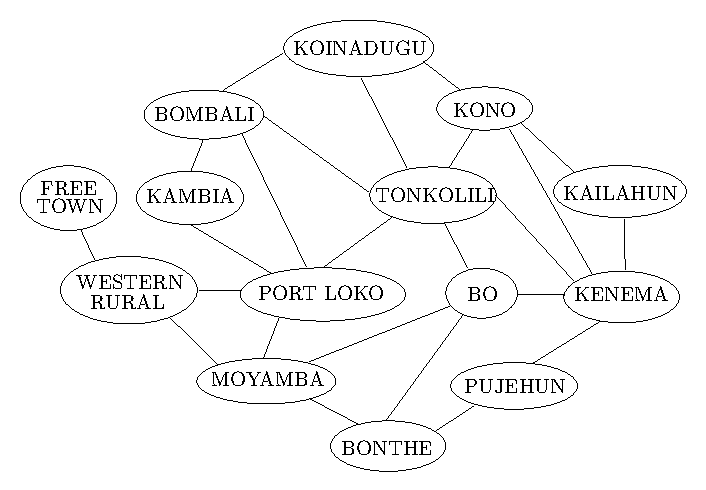
\includegraphics[width=11cm]{connectedgraph}
\caption{The connected graph of Seirra Leone}
\label{fig:connectedgraph}
\end{figure}



%================================GeneticAlgorithm==============================
\subsection{Genetic Algorithm}
Inspired by the process of natural selection, Genetic algorithm (GA) is routinely used to generate useful solutions to optimization and search problems. In our solution to the location of the delivery stations, we apply GA to determine the location according to the distances between neighboring districts and the latest epidemic situation.  

\subsubsection{Methodology}
In a genetic algorithm, a population of candidate solutions (called individuals, creatures, or phenotypes) to an optimization problem is evolved toward better solutions. Each candidate solution has a set of properties (its chromosomes or genotype) which can be mutated and altered; In our problem, solutions (number of the districts) are represented in binary.

The evolution usually starts from a population of randomly generated individuals, and is an iterative process. In each generation, the fitness of every individual usually (the value of the objective function ) in the population is evaluated; The more fit individuals are stochastically selected from the current population, and each individual's genome is modified (crossovered or mutated) to form a new generation. The new generation of candidate solutions is then used in the next iteration of the algorithm. Commonly, the algorithm terminates when the stop criteria is satisfied which is either a maximum number of generations has been produced, or a satisfactory fitness level has been reached for the population. The simplified process of GA is presented in \autoref{fig:GAprocess}.

\begin{figure}[ht]
\small
\centering
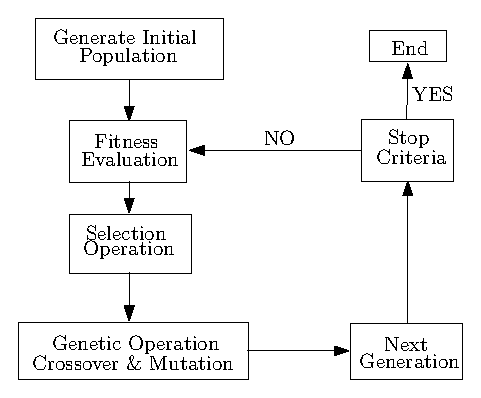
\includegraphics[width=9cm]{GAprocess}
\caption{The process of GA}
\label{fig:GAprocess}
\end{figure}

\subsubsection{Notations and numbering}

\begin{table}[h!]
\caption{Notations of GA} 
\medskip
\centering
\begin{tabular}{c c}
\hline
Definition & Symbol \\ [0.5ex]
\hline
the nearest station in $\{x,y,z\}$ to $i$ & $minS(i,x,y,z)$ \\
distance from $minS$ to $i$ & $minD(i,minS)$ \\
the amount of infected people in z & $In(z)$ \\

\hline
\end{tabular}
\label{t:notofGA}
\end{table}

\begin{table}[h!]
\caption{Numbering of the districts in Seirra\ Leone} 
\medskip
\centering
\begin{tabular}{c c c c c c c c}
\hline
Bo & Bombali & Bonthe & Freetown & Kailahun & Kambia & Kenema  \\ 
\hline
1 & 2& 3 & 4 & 5 & 6 & 7 \\ 
\hline
Koinadugu & Kono & Moyamba & Port\,Loko & Pujehun & Tonkolili & Western\,Rural  \\ 
\hline
8 & 9 & 10 & 11 & 12 & 13 & 14 \\ 
\hline
\end{tabular}

\label{t:numberingofSL}
\end{table}

\subsubsection{Application and solution}
As has been stated above, we apply GA to determine the location according the distances between neighboring districts and the latest epidemic situation. For instance, if only three main delivery station will be set up in Seirra Leone, the process of determination will be presented below.
First, we set the objective function in the optimization problem as:

$$min\ O(x,y,z)=\sum^{14}_{i=1}\frac {minD[\,minS(i,x,y,z)\,]}{In[\, minS(i,x,y,z)\,]}) $$
$$x,y,z\in\{Seirra\ Leone\}$$

Calculation        codes........
Solution       ........

4station  solution:...........


\subsection{Validating the model}%确认模型,使之合理。

\section{Interpretation}

\section{Discussion}

%================================总体评价==============================
\section{Evaluate of the model}

Like any model,the one present above has its strengths and
weaknesses. Some of the major points are presented below.

%============================模型=优点====================================
\subsection{Strengths}
\begin{itemize}
\item \textbf{Applies widely}\\
This  system can be used for many types of airplanes, and it also
solves the interference during  the procedure of the boarding
airplane,as described above we can get to the  optimization
boarding time.We also know that all the service is automate.
\item \textbf{Improve the quality of the airport service}\\
Balancing the cost of the cost and the benefit, it will bring in
more convenient  for airport and passengers.It also saves many
human resources for the airline. 
\end{itemize}
